%%%%%%%%%%%%%%%%%%%%%%%%%%%%%%%%%%%%%%%%%%%%%%%
% latex_template_ieee_bbing.tex
%
% 28.02.2008  bsb Created 
%%%%%%%%%%%%%%%%%%%%%%%%%%%%%%%%%%%%%%%%%%%%%%%%%

% Final - 2 column style
%\documentclass[10pt,final,journal]{../latexlib/latex_ieee/IEEEtran}
% Draft - single column style
\documentclass[11pt,draftcls,journal,onecolumn]{IEEEtran}

% If the IEEEtran.cls has not been installed into the LaTeX system files, 
% manually specify the path to it:
% \documentclass[conference]{../sty/IEEEtran} 

% Gives LaTeX2e the abilsity to do double column
%% correct bad hyphenation here
\hyphenation{op-tical net-works semi-conduc-tor IEEEtran}

% From thesis main (bbing)
\usepackage{amssymb,longtable,dcolumn}

% to use pdflatex
% Standard bbing packages
\usepackage{cite}      % Written by Donald Arseneau
\usepackage{graphicx}  % Written by David Carlisle and Sebastian Rahtz
\usepackage{url}       % Written by Donald Arseneau
\usepackage{amsmath, amssymb, longtable, dcolumn}
\usepackage{nccmath}  % Provides \medmath to change math size
\usepackage{bm}
%\usepackage{subfigure}
%\usepackage{stfloats}  % Written by Sigitas Tolusis
\usepackage[caption=false,font=footnotesize]{subfig}
%\usepackage{fixltx2e}
\usepackage{colortbl}
\usepackage{multirow}
\usepackage{amsmath}
\usepackage{units}
\usepackage{siunitx}
\usepackage{acronym}
\usepackage{csvsimple}
\usepackage{color,soul}

% Custom - need to be in the path
\usepackage{my_acronyms}
\usepackage{math_bbing}

% For using overleaf or local compilation
% See setting of true/false directly after \begin{document}
\newif\ifoverleaf % default is \overleaftrue

\begin{document}

\overleaffalse

\newtheorem{remark}{Remark}
\renewcommand{\theremark}{\unskip}


% List of new commands
% bbing 06-11-98

%\newcommand{\spacing}[1]{\renewcommand{\baselinestretch}{#1} \normalsize}

% Degree symbol within text
\newcommand{\degrees}{$^{\circ}$}
\newcommand{\CRlb}{Cram\'{e}r Rao }

\newcommand{\btab}{\begin{tabular}}
\newcommand{\etab}{\end{tabular}}

\newcommand{\bfig}{\begin{figure}}
\newcommand{\efig}{\end{figure}}

\newcommand{\beqn}{\begin{equation}}
\newcommand{\eeqn}{\end{equation}}
\newcommand{\bdm}{\begin{displaymath}}
\newcommand{\edm}{\end{displaymath}}

\newcommand{\bearray}{\begin{eqnarray}}
\newcommand{\eearray}{\end{eqnarray}}
\newcommand{\Bearray}{\begin{eqnarray}}
\newcommand{\Eearray}{\end{eqnarray}}

\newcommand{\bgat}{\begin{gather}}
\newcommand{\egat}{\end{gather}}

\newcommand{\Htwo}{$\mathcal{H}_2$\ }
\newcommand{\Hinf}{$\mathcal{H}_{\infty}$\ }

%\newcommand{\V}[1]{\mathbf{#1}}
\newcommand{\plusminus}{{\textstyle \frac{+}{-}}}

\newcommand{\TM}{$^{TM}$}

% Definitions  %from homero!
%
%\newcommand{\mtitle}[1]{\begin{center} {\huge \bf{#1}}\end{center}}
\newcommand{\lb}{\linebreak}
\newcommand{\xaxis}{\mbox{$x$-axis}}
\newcommand{\yaxis}{\mbox{$y$-axis}}
\newcommand{\zaxis}{\mbox{$z$-axis}}
\newcommand{\bc}{\begin{center}}
\newcommand{\ec}{\end{center}}
%\newcommand{\be}{\begin{equation}}
%\newcommand{\ee}{\end{equation}}
\newcommand{\bd}{\begin{displaymath}}
\newcommand{\ed}{\end{displaymath}}
\newcommand{\bi}{\begin{itemize}}
\newcommand{\ei}{\end{itemize}}
%\newcommand{\bt}{\begin{tabular}}
%\newcommand{\et}{\end{tabular}}
\newcommand{\ba}{\begin{array}}
\newcommand{\ea}{\end{array}}
\newcommand{\baa}[2]{\begin{array}[t]{cc}
\left[#1\right.\!\!&\!\!\left.#2\right]\end{array}} 
\newcommand{\bea}{\begin{eqnarray}}
\newcommand{\eea}{\end{eqnarray}}
\newcommand{\bsea}{\begin{subeqnarray}}
\newcommand{\esea}{\end{subeqnarray}}
\newcommand{\degr}{\mbox{$^{\circ}$}}
\newcommand{\jw}{j\omega}
\newcommand{\dw}{\mbox{\rm d}\omega}
\newcommand{\dx}[1]{\,\mbox{\rm d}#1}
\newcommand{\til}{^{\sim}}
\newcommand{\abcd}[4]{\left[\begin{array}{c|c}#1&#2\\ \hline #3&#4 
\end{array}\right]}
\newcommand{\etal}{{\em et al.}}
\newcommand{\etc}{{\em etc.}}
\newcommand{\eg}{{\em e.g., }}
\newcommand{\ie}{{\em i.e., }}
\newcommand{\eqnref}[1]{Equation~(\ref{#1})}
\newcommand{\eqrefa}[1]{Eq'n~(\ref{#1})}
\newcommand{\eqrefb}[1]{(\ref{#1})}
\newcommand{\expec}[1]{\left\langle #1 \right\rangle}
\newcommand{\pder}[2]{\frac{\partial #1}{\partial #2}}
\newcommand{\half}{{\textstyle \frac{1}{2}}}
\newcommand{\msp}{\mbox{\hspace{.5in}}}
\newcommand{\ub}[2]{\underbrace{#1}_{#2}}
\newcommand{\eqn}[1]{Eq.~\ref{eq:#1}}
%
%\newenvironment{proof}{\par\noindent{\bf Proof: }}{\hfill $\Box$}
%\newenvironment{remark}{{\bf Remark: }}{}
%
\def\sinc{\mathop{\rm sinc}\nolimits}
%
\newcommand{\vdashes}[2]
   {{\vfuzz #1 \vbox to 0pt{\vskip -#2
   \vbox{\xleaders\vbox{\vskip 1pt\hfuzz 1pt\hbox to 0pt{\vrule height 4pt
   depth 0pt}\vskip 1pt}\vskip #1}}}}


\newcommand{\bmat}[1]{\left[ \begin{array}{#1}}
\newcommand{\emat}{\end{array} \right]}
%\newcommand{\bvec}{\left( \begin{array}{c}}
\newcommand{\evec}{\end{array} \right)}

  % shortcuts to thesis stuff
% Stolen from Austratlian Center for Field Robotics
% Thanks Alex!
% bbing 24.02.03

% references to figurs and equations
\newcommand{\fref}[1] {Figure~\ref{#1}}
\newcommand{\eref}[1] {~(\ref{#1})}

% general global definitions
\newcommand{\Def}{\ {\buildrel \triangle\over =}\ }
%\newcommand{\beq} {\begin{equation}}
%\newcommand{\eeq} {\end{equation}}
%\newcommand{\beqn} {\begin{eqnarray}}
%\newcommand{\eeqn} {\end{eqnarray}}
%\newcommand{\E}[1] {\mbox{$ {\rm E} \{ #1 \}$ }}
\newcommand{\Es}[2] {\mbox{$ {\rm E}^{#1} \{ #2 \}$ }}
\newcommand{\Set}[1] {\mbox{$ \{ #1 \} $ }}
\newcommand{\Cal}[1] {\mbox{$ {\cal #1 } $}}
\newcommand{\PR}[1]  {\mbox{$ P(#1) $}}
\newcommand{\Pri}[2]  {\mbox{$ P_{#1}(#2) $}}
\newcommand{\PRi}[2]  {\mbox{$ P_{#1}(#2) $}}
\newcommand{\Pris}[3]  {\mbox{$ P_{#1}^{#2}(#3) $}}
\newcommand{\like}[1]  {\mbox{$ \Lambda(\bf #1) $}}
\newcommand{\likei}[2]  {\mbox{$ \Lambda_{#2}(\bf #1) $}}
\newcommand{\LL}[1]  {\mbox{$ l(#1) $}} % loglikelihood
\newcommand{\LLi}[2]  {\mbox{$ l_{#1}(#2) $}} %loglikelihood
\newcommand{\EN}[1]  {\mbox{$ H(#1) $}} % entropy
\newcommand{\ENi}[2]  {\mbox{$ H_{#1}(#2) $}} % entropy
\newcommand{\mEN}[1]  {\mbox{$ \overline{H}(#1) $}} % mean entropy
\newcommand{\MI}[1]  {\mbox{$ I(#1) $}}  %mutual information
\newcommand{\est}[1]  {\mbox{$\hat{\bf #1}$}}
\newcommand{\estk}[2]  {\mbox{$\hat{\bf #1}(#2)$}}
\newcommand{\D}[1]    {\mbox{${\rm d} {#1}$}}
\newcommand{\mean}[1] {\mbox{$\overline{ #1}$}}
\newcommand{\Det}[1] {\mbox{$\mid {#1} \mid $}}
\newcommand{\One}      {\mbox{${\bf 1}$}}
\newcommand{\Zero}      {\mbox{${\bf 0}$}}
\newcommand{\grad}[1] {\mbox{${\bf\nabla} #1$}}
\newcommand{\J}[3] {\mbox{${\bf\nabla}{\bf #1}_{\bf #2}(#3)$}}
\newcommand{\Jt}[3] {\mbox{${\bf\nabla}^T{\bf #1}_{\bf #2}(#3)$}}
\newcommand{\pdf}{{\it pdf\ }}
\newcommand{\dxt}[2]  {\mbox{$\dot{\bf #1}( #2)$}}
% defining different types of vectors
% first those with no time subscripts
\newcommand{\V}[1] {\mbox{${\bf #1}$}}
\newcommand{\Vt}[1] {\mbox{${\bf #1}^T$}}
\newcommand{\Vin}[1] {\mbox{${\bf #1}^{-1}$}}
\newcommand{\Vgin}[1] {\mbox{${\bf #1}^{\dagger}$}}
\newcommand{\Vi}[2] {\mbox{${\bf #1}_{#2}$}}
\newcommand{\Vs}[2] {\mbox{${\bf #1}^{#2}$}}
\newcommand{\Vis}[3] {\mbox{${\bf #1}_{#2}^{#3}$}}
\newcommand{\Vit}[2] {\mbox{${\bf #1}_{#2}^T$}}
\newcommand{\Vini}[2] {\mbox{${\bf #1}_{#2}^{-1}$}}
\newcommand{\Vgini}[2] {\mbox{${\bf #1}^{\dagger}$}}

% next those with time subscript k (very common)
\newcommand{\Vk}[1] {\mbox{${\bf #1}(k)$}}
\newcommand{\Vkt}[1] {\mbox{${\bf #1}^T(k)$}}
\newcommand{\Vkin}[1] {\mbox{${\bf #1}^{-1}(k)$}}
\newcommand{\Vkgin}[1] {\mbox{${\bf #1}^{\dagger}(k)$}}
\newcommand{\Vki}[2] {\mbox{${\bf #1}_{#2}(k)$}}
\newcommand{\Vks}[2] {\mbox{${\bf #1}^{#2}(k)$}}
\newcommand{\Vkis}[3] {\mbox{${\bf #1}_{#2}^{#3}(k)$}}
\newcommand{\Vkit}[2] {\mbox{${\bf #1}_{#2}^T(k)$}}
\newcommand{\Vkini}[2] {\mbox{${\bf #1}_{#2}^{-1}(k)$}}
\newcommand{\Vkgini}[2] {\mbox{${\bf #1}^{\dagger}_{#2}(k)$}}
\newcommand{\tVk}[1] {\mbox{$\tilde{\bf #1}(k)$}}
\newcommand{\tVki}[2] {\mbox{$\tilde{\bf #1}_{#2}(k)$}}

% now those with general purpose time subscripts
%\newcommand{\Vec}[2] {\mbox{${\bf #1}(#2)$}}
\newcommand{\Vect}[2] {\mbox{${\bf #1}^T(#2)$}}
\newcommand{\Vecin}[2] {\mbox{${\bf #1}^{-1}(#2)$}}
\newcommand{\Veci}[3] {\mbox{${\bf #1}_{#2}(#3)$}}
\newcommand{\Vecit}[3] {\mbox{${\bf #1}_{#2}^T(#3)$}}
\newcommand{\Vecini}[3] {\mbox{${\bf #1}_{#2}^{-1}(#3)$}}
\newcommand{\Vecgin}[2] {\mbox{${\bf #1}^{\dagger}(#2)$}}
\newcommand{\Vecgini}[3] {\mbox{${\bf #1}^{\dagger}_{#2}(#3)$}}

% special symbols used very commonly
% state estimates of different sorts
\newcommand{\x}[2] {\mbox{$\hat{\bf x}( #1 \mid #2)$}}
\newcommand{\ix}[3] {\mbox{$\hat{\bf x}_{#1}( #2 \mid #3)$}}
\newcommand{\tx}[2] {\mbox{$\tilde{\bf x}( #1 \mid #2 )$}}
\newcommand{\txi}[3] {\mbox{$\tilde{\bf x}_{#1}( #2 \mid #3 )$}}
\newcommand{\z}[2] {\mbox{$\hat{\bf z}( #1 \mid #2)$}}
\newcommand{\tz}[2] {\mbox{$\tilde{\bf z}( #1 \mid #2)$}}
\newcommand{\tzt}[2] {\mbox{$\tilde{\bf z}^T( #1 \mid #2)$}}
\newcommand{\zi}[3] {\mbox{$\hat{\bf z}_{#1}( #2 \mid #3)$}}
\newcommand{\di}[3] {\mbox{$\hat{\bf \delta}_{#1}( #2 \mid #3)$}}

% variances of different sorts
\newcommand{\var}[2] {\mbox{${\bf P}( #1 \mid #2)$}}
\newcommand{\varin}[2] {\mbox{${\bf P}^{-1}( #1 \mid #2)$}}
\newcommand{\tvar}[2] {\mbox{$\tilde{\bf P}( #1 \mid #2)$}}
\newcommand{\tvarin}[2] {\mbox{$\tilde{\bf P}^{-1}( #1 \mid #2)$}}
\newcommand{\vari}[3] {\mbox{${\bf P}_{#1}( #2 \mid #3)$}}
\newcommand{\varini}[3] {\mbox{${\bf P}^{-1}_{#1}( #2 \mid #3)$}}
\newcommand{\tvari}[3] {\mbox{$\tilde{\bf P}_{#1}( #2 \mid #3)$}}
\newcommand{\tvarini}[3] {\mbox{$\tilde{\bf P}^{-1}_{#1}( #2 \mid #3)$}}

% information states and variances
\newcommand{\y}[2] {\mbox{$\hat{\bf y}( #1 \mid #2)$}}
\newcommand{\ty}[2] {\mbox{$\tilde{\bf y}( #1 \mid #2)$}}
\newcommand{\yi}[3] {\mbox{$\hat{\bf y}_{#1}( #2 \mid #3)$}}
\newcommand{\tyi}[3] {\mbox{$\tilde{\bf y}_{#1}( #2 \mid #3)$}}
\newcommand{\Y}[2] {\mbox{${\bf Y}( #1 \mid #2)$}}
\newcommand{\Yin}[2] {\mbox{${\bf Y}^{-1}( #1 \mid #2)$}}
\newcommand{\tY}[2] {\mbox{$\tilde{\bf Y}( #1 \mid #2)$}}
\newcommand{\Yi}[3] {\mbox{${\bf Y}_{#1}( #2 \mid #3)$}}
\newcommand{\Yini}[3] {\mbox{${\bf Y}_{#1}^{-1}( #2 \mid #3)$}}
\newcommand{\tYi}[3] {\mbox{$\tilde{\bf Y}_{#1}( #2 \mid #3)$}}
\newcommand{\info}[1] {\mbox{${\bf i}( #1)$}}
\newcommand{\Info}[1] {\mbox{${\bf I}( #1)$}}
\newcommand{\infoi}[2] {\mbox{${\bf i}_{#1}( #2)$}}
\newcommand{\infois}[3] {\mbox{${\bf i}_{#1}^{#2}(#3)$}}
\newcommand{\Infoi}[2] {\mbox{${\bf I}_{#1}( #2)$}}
\newcommand{\tInfoi}[2] {\mbox{$\tilde{\bf I}_{#1}( #2)$}}
\newcommand{\Infoini}[2] {\mbox{${\bf I}^{\dagger}_{#1}( #2)$}}
\newcommand{\Prop}[2] {\mbox{${\bf L}( #1 \mid #2)$}}
\newcommand{\Propi}[3] {\mbox{${\bf L}_{#1}( #2 \mid #3)$}}
\newcommand{\Z}[2] {\mbox{${\cal Z}^{#1}_{#2}$}}

% spurious ones
\newcommand{\maybe}{\ {\buildrel ?\over =}\ } %chapter 4
\newcommand{\svd} {\mbox{$\dagger$}} % chapter 4
\newcommand{\dnoise} {\mbox{$\delta d$}} % chapter 6 and 7
\newcommand{\unoise} {\mbox{$\delta u$}} % chapter 6
\newcommand{\ns}[1] {\mbox{$ #1$}} % chapter 6
\newcommand{\vs} {\vspace{0.17in}}
\newcommand{\svs} {\vspace{0.17cm}}
\newcommand{\vsf} {\vspace{0.4in}}
\newcommand{\vsff} {\vspace{1in}}
\newcommand{\veqns} {\vspace{-0.15in}}
\newcommand{\veqn} {\vspace{-0.12in}}
\newcommand{\sveqn} {\vspace{-0.06in}}
%\newcommand{\bc}{\begin{center}}
%\newcommand{\ec}{\end{center}}
%\newcommand{\bi}{\begin{itemize}}
%\newcommand{\ei}{\end{itemize}}
%\newcommand{\be}{\begin{enumerate}}
%\newcommand{\ee}{\end{enumerate}}
\newcommand{\Quote}{\parbox[t]{12.5cm}}
\newtheorem{example}{Example}

%% List of new commands
% bbing 06-11-98

%\newcommand{\spacing}[1]{\renewcommand{\baselinestretch}{#1} \normalsize}

% Degree symbol within text
\newcommand{\degrees}{$^{\circ}$}
\newcommand{\CRlb}{Cram\'{e}r Rao }

\newcommand{\btab}{\begin{tabular}}
\newcommand{\etab}{\end{tabular}}

\newcommand{\bfig}{\begin{figure}}
\newcommand{\efig}{\end{figure}}

\newcommand{\beqn}{\begin{equation}}
\newcommand{\eeqn}{\end{equation}}
\newcommand{\bdm}{\begin{displaymath}}
\newcommand{\edm}{\end{displaymath}}

\newcommand{\bearray}{\begin{eqnarray}}
\newcommand{\eearray}{\end{eqnarray}}
\newcommand{\Bearray}{\begin{eqnarray}}
\newcommand{\Eearray}{\end{eqnarray}}

\newcommand{\bgat}{\begin{gather}}
\newcommand{\egat}{\end{gather}}

\newcommand{\Htwo}{$\mathcal{H}_2$\ }
\newcommand{\Hinf}{$\mathcal{H}_{\infty}$\ }

%\newcommand{\V}[1]{\mathbf{#1}}
\newcommand{\plusminus}{{\textstyle \frac{+}{-}}}

\newcommand{\TM}{$^{TM}$}

% Definitions  %from homero!
%
%\newcommand{\mtitle}[1]{\begin{center} {\huge \bf{#1}}\end{center}}
\newcommand{\lb}{\linebreak}
\newcommand{\xaxis}{\mbox{$x$-axis}}
\newcommand{\yaxis}{\mbox{$y$-axis}}
\newcommand{\zaxis}{\mbox{$z$-axis}}
\newcommand{\bc}{\begin{center}}
\newcommand{\ec}{\end{center}}
%\newcommand{\be}{\begin{equation}}
%\newcommand{\ee}{\end{equation}}
\newcommand{\bd}{\begin{displaymath}}
\newcommand{\ed}{\end{displaymath}}
\newcommand{\bi}{\begin{itemize}}
\newcommand{\ei}{\end{itemize}}
%\newcommand{\bt}{\begin{tabular}}
%\newcommand{\et}{\end{tabular}}
\newcommand{\ba}{\begin{array}}
\newcommand{\ea}{\end{array}}
\newcommand{\baa}[2]{\begin{array}[t]{cc}
\left[#1\right.\!\!&\!\!\left.#2\right]\end{array}} 
\newcommand{\bea}{\begin{eqnarray}}
\newcommand{\eea}{\end{eqnarray}}
\newcommand{\bsea}{\begin{subeqnarray}}
\newcommand{\esea}{\end{subeqnarray}}
\newcommand{\degr}{\mbox{$^{\circ}$}}
\newcommand{\jw}{j\omega}
\newcommand{\dw}{\mbox{\rm d}\omega}
\newcommand{\dx}[1]{\,\mbox{\rm d}#1}
\newcommand{\til}{^{\sim}}
\newcommand{\abcd}[4]{\left[\begin{array}{c|c}#1&#2\\ \hline #3&#4 
\end{array}\right]}
\newcommand{\etal}{{\em et al.}}
\newcommand{\etc}{{\em etc.}}
\newcommand{\eg}{{\em e.g., }}
\newcommand{\ie}{{\em i.e., }}
\newcommand{\eqnref}[1]{Equation~(\ref{#1})}
\newcommand{\eqrefa}[1]{Eq'n~(\ref{#1})}
\newcommand{\eqrefb}[1]{(\ref{#1})}
\newcommand{\expec}[1]{\left\langle #1 \right\rangle}
\newcommand{\pder}[2]{\frac{\partial #1}{\partial #2}}
\newcommand{\half}{{\textstyle \frac{1}{2}}}
\newcommand{\msp}{\mbox{\hspace{.5in}}}
\newcommand{\ub}[2]{\underbrace{#1}_{#2}}
\newcommand{\eqn}[1]{Eq.~\ref{eq:#1}}
%
%\newenvironment{proof}{\par\noindent{\bf Proof: }}{\hfill $\Box$}
%\newenvironment{remark}{{\bf Remark: }}{}
%
\def\sinc{\mathop{\rm sinc}\nolimits}
%
\newcommand{\vdashes}[2]
   {{\vfuzz #1 \vbox to 0pt{\vskip -#2
   \vbox{\xleaders\vbox{\vskip 1pt\hfuzz 1pt\hbox to 0pt{\vrule height 4pt
   depth 0pt}\vskip 1pt}\vskip #1}}}}


\newcommand{\bmat}[1]{\left[ \begin{array}{#1}}
\newcommand{\emat}{\end{array} \right]}
%\newcommand{\bvec}{\left( \begin{array}{c}}
\newcommand{\evec}{\end{array} \right)}

  % shortcuts to thesis stuff
%% Stolen from Austratlian Center for Field Robotics
% Thanks Alex!
% bbing 24.02.03

% references to figurs and equations
\newcommand{\fref}[1] {Figure~\ref{#1}}
\newcommand{\eref}[1] {~(\ref{#1})}

% general global definitions
\newcommand{\Def}{\ {\buildrel \triangle\over =}\ }
%\newcommand{\beq} {\begin{equation}}
%\newcommand{\eeq} {\end{equation}}
%\newcommand{\beqn} {\begin{eqnarray}}
%\newcommand{\eeqn} {\end{eqnarray}}
%\newcommand{\E}[1] {\mbox{$ {\rm E} \{ #1 \}$ }}
\newcommand{\Es}[2] {\mbox{$ {\rm E}^{#1} \{ #2 \}$ }}
\newcommand{\Set}[1] {\mbox{$ \{ #1 \} $ }}
\newcommand{\Cal}[1] {\mbox{$ {\cal #1 } $}}
\newcommand{\PR}[1]  {\mbox{$ P(#1) $}}
\newcommand{\Pri}[2]  {\mbox{$ P_{#1}(#2) $}}
\newcommand{\PRi}[2]  {\mbox{$ P_{#1}(#2) $}}
\newcommand{\Pris}[3]  {\mbox{$ P_{#1}^{#2}(#3) $}}
\newcommand{\like}[1]  {\mbox{$ \Lambda(\bf #1) $}}
\newcommand{\likei}[2]  {\mbox{$ \Lambda_{#2}(\bf #1) $}}
\newcommand{\LL}[1]  {\mbox{$ l(#1) $}} % loglikelihood
\newcommand{\LLi}[2]  {\mbox{$ l_{#1}(#2) $}} %loglikelihood
\newcommand{\EN}[1]  {\mbox{$ H(#1) $}} % entropy
\newcommand{\ENi}[2]  {\mbox{$ H_{#1}(#2) $}} % entropy
\newcommand{\mEN}[1]  {\mbox{$ \overline{H}(#1) $}} % mean entropy
\newcommand{\MI}[1]  {\mbox{$ I(#1) $}}  %mutual information
\newcommand{\est}[1]  {\mbox{$\hat{\bf #1}$}}
\newcommand{\estk}[2]  {\mbox{$\hat{\bf #1}(#2)$}}
\newcommand{\D}[1]    {\mbox{${\rm d} {#1}$}}
\newcommand{\mean}[1] {\mbox{$\overline{ #1}$}}
\newcommand{\Det}[1] {\mbox{$\mid {#1} \mid $}}
\newcommand{\One}      {\mbox{${\bf 1}$}}
\newcommand{\Zero}      {\mbox{${\bf 0}$}}
\newcommand{\grad}[1] {\mbox{${\bf\nabla} #1$}}
\newcommand{\J}[3] {\mbox{${\bf\nabla}{\bf #1}_{\bf #2}(#3)$}}
\newcommand{\Jt}[3] {\mbox{${\bf\nabla}^T{\bf #1}_{\bf #2}(#3)$}}
\newcommand{\pdf}{{\it pdf\ }}
\newcommand{\dxt}[2]  {\mbox{$\dot{\bf #1}( #2)$}}
% defining different types of vectors
% first those with no time subscripts
\newcommand{\V}[1] {\mbox{${\bf #1}$}}
\newcommand{\Vt}[1] {\mbox{${\bf #1}^T$}}
\newcommand{\Vin}[1] {\mbox{${\bf #1}^{-1}$}}
\newcommand{\Vgin}[1] {\mbox{${\bf #1}^{\dagger}$}}
\newcommand{\Vi}[2] {\mbox{${\bf #1}_{#2}$}}
\newcommand{\Vs}[2] {\mbox{${\bf #1}^{#2}$}}
\newcommand{\Vis}[3] {\mbox{${\bf #1}_{#2}^{#3}$}}
\newcommand{\Vit}[2] {\mbox{${\bf #1}_{#2}^T$}}
\newcommand{\Vini}[2] {\mbox{${\bf #1}_{#2}^{-1}$}}
\newcommand{\Vgini}[2] {\mbox{${\bf #1}^{\dagger}$}}

% next those with time subscript k (very common)
\newcommand{\Vk}[1] {\mbox{${\bf #1}(k)$}}
\newcommand{\Vkt}[1] {\mbox{${\bf #1}^T(k)$}}
\newcommand{\Vkin}[1] {\mbox{${\bf #1}^{-1}(k)$}}
\newcommand{\Vkgin}[1] {\mbox{${\bf #1}^{\dagger}(k)$}}
\newcommand{\Vki}[2] {\mbox{${\bf #1}_{#2}(k)$}}
\newcommand{\Vks}[2] {\mbox{${\bf #1}^{#2}(k)$}}
\newcommand{\Vkis}[3] {\mbox{${\bf #1}_{#2}^{#3}(k)$}}
\newcommand{\Vkit}[2] {\mbox{${\bf #1}_{#2}^T(k)$}}
\newcommand{\Vkini}[2] {\mbox{${\bf #1}_{#2}^{-1}(k)$}}
\newcommand{\Vkgini}[2] {\mbox{${\bf #1}^{\dagger}_{#2}(k)$}}
\newcommand{\tVk}[1] {\mbox{$\tilde{\bf #1}(k)$}}
\newcommand{\tVki}[2] {\mbox{$\tilde{\bf #1}_{#2}(k)$}}

% now those with general purpose time subscripts
%\newcommand{\Vec}[2] {\mbox{${\bf #1}(#2)$}}
\newcommand{\Vect}[2] {\mbox{${\bf #1}^T(#2)$}}
\newcommand{\Vecin}[2] {\mbox{${\bf #1}^{-1}(#2)$}}
\newcommand{\Veci}[3] {\mbox{${\bf #1}_{#2}(#3)$}}
\newcommand{\Vecit}[3] {\mbox{${\bf #1}_{#2}^T(#3)$}}
\newcommand{\Vecini}[3] {\mbox{${\bf #1}_{#2}^{-1}(#3)$}}
\newcommand{\Vecgin}[2] {\mbox{${\bf #1}^{\dagger}(#2)$}}
\newcommand{\Vecgini}[3] {\mbox{${\bf #1}^{\dagger}_{#2}(#3)$}}

% special symbols used very commonly
% state estimates of different sorts
\newcommand{\x}[2] {\mbox{$\hat{\bf x}( #1 \mid #2)$}}
\newcommand{\ix}[3] {\mbox{$\hat{\bf x}_{#1}( #2 \mid #3)$}}
\newcommand{\tx}[2] {\mbox{$\tilde{\bf x}( #1 \mid #2 )$}}
\newcommand{\txi}[3] {\mbox{$\tilde{\bf x}_{#1}( #2 \mid #3 )$}}
\newcommand{\z}[2] {\mbox{$\hat{\bf z}( #1 \mid #2)$}}
\newcommand{\tz}[2] {\mbox{$\tilde{\bf z}( #1 \mid #2)$}}
\newcommand{\tzt}[2] {\mbox{$\tilde{\bf z}^T( #1 \mid #2)$}}
\newcommand{\zi}[3] {\mbox{$\hat{\bf z}_{#1}( #2 \mid #3)$}}
\newcommand{\di}[3] {\mbox{$\hat{\bf \delta}_{#1}( #2 \mid #3)$}}

% variances of different sorts
\newcommand{\var}[2] {\mbox{${\bf P}( #1 \mid #2)$}}
\newcommand{\varin}[2] {\mbox{${\bf P}^{-1}( #1 \mid #2)$}}
\newcommand{\tvar}[2] {\mbox{$\tilde{\bf P}( #1 \mid #2)$}}
\newcommand{\tvarin}[2] {\mbox{$\tilde{\bf P}^{-1}( #1 \mid #2)$}}
\newcommand{\vari}[3] {\mbox{${\bf P}_{#1}( #2 \mid #3)$}}
\newcommand{\varini}[3] {\mbox{${\bf P}^{-1}_{#1}( #2 \mid #3)$}}
\newcommand{\tvari}[3] {\mbox{$\tilde{\bf P}_{#1}( #2 \mid #3)$}}
\newcommand{\tvarini}[3] {\mbox{$\tilde{\bf P}^{-1}_{#1}( #2 \mid #3)$}}

% information states and variances
\newcommand{\y}[2] {\mbox{$\hat{\bf y}( #1 \mid #2)$}}
\newcommand{\ty}[2] {\mbox{$\tilde{\bf y}( #1 \mid #2)$}}
\newcommand{\yi}[3] {\mbox{$\hat{\bf y}_{#1}( #2 \mid #3)$}}
\newcommand{\tyi}[3] {\mbox{$\tilde{\bf y}_{#1}( #2 \mid #3)$}}
\newcommand{\Y}[2] {\mbox{${\bf Y}( #1 \mid #2)$}}
\newcommand{\Yin}[2] {\mbox{${\bf Y}^{-1}( #1 \mid #2)$}}
\newcommand{\tY}[2] {\mbox{$\tilde{\bf Y}( #1 \mid #2)$}}
\newcommand{\Yi}[3] {\mbox{${\bf Y}_{#1}( #2 \mid #3)$}}
\newcommand{\Yini}[3] {\mbox{${\bf Y}_{#1}^{-1}( #2 \mid #3)$}}
\newcommand{\tYi}[3] {\mbox{$\tilde{\bf Y}_{#1}( #2 \mid #3)$}}
\newcommand{\info}[1] {\mbox{${\bf i}( #1)$}}
\newcommand{\Info}[1] {\mbox{${\bf I}( #1)$}}
\newcommand{\infoi}[2] {\mbox{${\bf i}_{#1}( #2)$}}
\newcommand{\infois}[3] {\mbox{${\bf i}_{#1}^{#2}(#3)$}}
\newcommand{\Infoi}[2] {\mbox{${\bf I}_{#1}( #2)$}}
\newcommand{\tInfoi}[2] {\mbox{$\tilde{\bf I}_{#1}( #2)$}}
\newcommand{\Infoini}[2] {\mbox{${\bf I}^{\dagger}_{#1}( #2)$}}
\newcommand{\Prop}[2] {\mbox{${\bf L}( #1 \mid #2)$}}
\newcommand{\Propi}[3] {\mbox{${\bf L}_{#1}( #2 \mid #3)$}}
\newcommand{\Z}[2] {\mbox{${\cal Z}^{#1}_{#2}$}}

% spurious ones
\newcommand{\maybe}{\ {\buildrel ?\over =}\ } %chapter 4
\newcommand{\svd} {\mbox{$\dagger$}} % chapter 4
\newcommand{\dnoise} {\mbox{$\delta d$}} % chapter 6 and 7
\newcommand{\unoise} {\mbox{$\delta u$}} % chapter 6
\newcommand{\ns}[1] {\mbox{$ #1$}} % chapter 6
\newcommand{\vs} {\vspace{0.17in}}
\newcommand{\svs} {\vspace{0.17cm}}
\newcommand{\vsf} {\vspace{0.4in}}
\newcommand{\vsff} {\vspace{1in}}
\newcommand{\veqns} {\vspace{-0.15in}}
\newcommand{\veqn} {\vspace{-0.12in}}
\newcommand{\sveqn} {\vspace{-0.06in}}
%\newcommand{\bc}{\begin{center}}
%\newcommand{\ec}{\end{center}}
%\newcommand{\bi}{\begin{itemize}}
%\newcommand{\ei}{\end{itemize}}
%\newcommand{\be}{\begin{enumerate}}
%\newcommand{\ee}{\end{enumerate}}
\newcommand{\Quote}{\parbox[t]{12.5cm}}
\newtheorem{example}{Example}



% set the figure default size
\newcommand{\SF}{0.2}
\newcommand{\SFb}{0.45}
\newcommand{\SFPic}{0.45}
\newcommand{\SFPlot}{0.45}
\newcommand{\SFc}{0.25}
% Just a lazy way of setting the figure width (percentage of text width)
% 0.7 works well for 1 column
% 0.4 works well for 2 column
\newcommand{\FigWidth}{\SFb}

% Use this one for the draft version
\newcommand{\scaleOneTwo}[2] {\scalebox{#1}}
% Use this one for the two column version
%\newcommand{\scaleOneTwo}[2] {\scalebox{#2}}

% Graphics for this paper
\graphicspath{{images/}}

% paper title
%\title{Towards an Experimentally Validated Plume Model to Support Robotic Plume Characterization}
\title{USV Modeling}

% author names and affiliations
% use a multiple column layout for up to three different
% affiliations
\author{Brian~Bingham$^{1}$% <-this % stops a space
\thanks{$^{1}$ Brian~Bingham is with the Department of Mechanical and Aerospace Engineering, Naval Postgraduate School, Monterey, CA 93950, USA. {\tt\small bbingham@nps.edu}}%
}

% make the title area
\maketitle

%\begin{abstract}
%Abstract
%\end{abstract}
% no keywords

\IEEEpeerreviewmaketitle

\section{Introduction}
The goal of this effort is to develop a USV model that 
\begin{itemize}
\item Is appropriate for design and evaluation of control algorithms
\item Balances fidelity with capacity for empirical parameter estimation
\item Can be identified using static tests and maneuvering trials with a USV and on board sensors
\item Makes use of physically measurable quantities (mass and inertia)
\item Enables prediction of dynamics with and without water current
\end{itemize} 

\section{Background}

Below is a survey of a small number of the relevant prior work on modeling USVs for control.  

\subsection{\cite{fossen94guidance} and \cite{fossen11handbook}}
The maneuvering models described by Fossen appear to be the basis for most of the USV work.  The references contain a number of different generic models and extensions of these models for specific cases.  The focus tends to be on full-sized surface ships and platforms, but are relevant to small USVs. 

\subsection{\cite{sonnenburg10control} and \cite{sonnenburg13modeling}}

\cite{sonnenburg13modeling} and \cite{sonnenburg10control} examine model for USV with steerable outboard motor (vectored thrust) where sideslip is a major concern.  Uses notation and maneuvering model from \cite{fossen94guidance}.
\begin{itemize}
\item Full vessel model is includes linear and quadratic damping
\item All models are then linearized (perturbation dynamics) for the purpose of identification where the coefficients are parameterized by the states (surge, sway and yaw-rate)
\item Actuation model thrust as a linear  and quadratic with velocity dependence.
\end{itemize}
Model identification appears to throw out the physical model and rely on identification of linear models (perturbation models) and a set of discrete speeds.
\begin{itemize}
\item Model identification includes open-loop maneuvers to identify steady-state parameters and closed-loop maneuvers to identify dynamic parameters.
\begin{enumerate}
\item Steady-state values are identified by as linear relationships between yaw-rate, side-slip angle and side-sleep speed.  The coefficients of these a relationships are determined for a set of discrete, constant speeds.  The values of these coefficients change significantly over the range of forward speeds and now functional relationship is offered.  
\item Thruster model conflates both the thrust relationship and the inertia of the system.  Model is identified by measuring initial acceleration during step changes in engine RPM and identifying the two linear coefficients of a linear model.  This single model is constant over the range of speeds.  Sparse data at higher speeds.
\item Speed/surge is modeled as first-order model parameterized over speed range.
\item Steering model (first order Nomoto model with sideslip) is identified by minimizing a quadratic cost function of sideslip angle and yaw-rate over close-loop time histories. Again, the linearized models have coefficients that change with speed.  The results again show significant changes over the speed envelope without offering a functional relationship.
\end{enumerate}
\end{itemize}

\subsection{\cite{caccia08practical}}
Uses the nonlinear model of Blanke \cite{blanke81ship} as reported in \cite{fossen94guidance}.  Speed/surge model:
\begin{itemize}
\item Neglects added mass term based on Blanke comments.  Blanke suggests that the surge added mass term ``will typically be less then 5\%'' \cite{fossen94guidance}.
\item Neglects $r^2$ terms, as suggested by Blanke, based on assuming reasonable low yaw-rate (< 10 degrees/s). 
\item Assumes linear+quadratic drag.  The Blanke model reported in \cite{fossen94guidance} includes only the quadratic term.  
\item Neglects the Coriolis terms based on assuming negligible sway velocity.  The experimental evidence from \cite{sonnenburg13modeling} and \cite{sonnenburg10control} indicate that there is a significant sideslip angle, hence a significant sway velocity.
\end{itemize}
Steering model
\begin{itemize}
\item Neglects added mass in surge and yaw.
\end{itemize}
Sway (sideslip) was not observable in experiments!  Used only GPS and heading for identification making making many of the estimated quantities unreliable or unobservable.

Thrust model neglects speed of advance, assumes thrust is independent of vessel speed.

\section{Simplified Maneuvering Models for Control}
The horizontal-plane \emph{maneuvering model} uses the state vector $\bm{\nu}=[u,v,r]^T$ where the velocities $u$, $v$ and $r$ are in the surge, sway and yaw directions respectively. 

Euler angles for angular displacements/velocities are
\begin{itemize}
\item roll $\phi$, $p=\dot{\phi}$
\item pitch $\theta$, $q=\dot{\theta}$
\item yaw $\psi$, $r=\dot{\psi}$
\end{itemize}

We consider control to regulate the forward speed ($u$) and the yaw angle ($\psi$) simultaneously, but for simplicity we will consider surge and yaw independently.  This allows us to develop single-input, single-output control designs for each degree-of-freedom independently, and them combine them in the implementation.

\subsection{Linear Models of Surge and Yaw}
This is the simplest model and us useful as a benchmark for control performance.
\begin{itemize}
\item linear dynamics
\item linear thrust model
\item unbounded thrust
\item uncoupled dynamics (surge/sway/yaw)
\end{itemize}

Control inputs:
\begin{itemize}
\item $X_c$ is total control force in the surge direction.
\item $N_c$ is the total control torque in the yaw direction.
\end{itemize}

Surge model
\[
m \dot{u} + X_u u = X_c
\]
where $m$ is the total mass, both rigid body and added mass, and $X_u$ is the linear drag.

Yaw model
\[
I_z \ddot{\psi} + N_r \dot{\psi} = N_c
\]
where $I_z$ is the total inertia in the yaw direction and $N_r$ is the linear drag.

Here are some rough physical parameters to use.
\begin{itemize}
\item $m=\unit[28]{kg}$: based on weight specified by clearpath.  Ignores added-mass.  Should weigh our actual USV to verify.
\item $X_u=\frac{\unitfrac[1.5]{m}{s}}{\unit[40]{N}}=\unitfrac[0.0375]{m}{Ns}$: based on linear interpretation of Figure~\ref{f:t-force}.
\item $I_z = \unit[28]{kg} (\unit[0.5]{m})^2 = \unit[6.25]{kg m^2}$: based on approximation of USV as thin disc.
\item $N_r = \frac{\unitfrac[0.25]{rad}{s}}{\unit{8}{Nm}} = \unitfrac[0.0313]{rad}{Nms}$: basded on linear interpretation of Figure~\ref{f:t-yaw}.
\end{itemize}

\subsubsection{Linear Model Control: PID}

With this specific model, we can apply build a two PID controllers - one for the surge model (PI control) and one of the yaw model (PD control).  Use Zeigler-Nichols, or similar, tuning process to standardize the tuning.  Use this as a baseline for closed-loop performance.

\subsubsection{Linear Model Control: PID+}
Consider adding a feedforward term to the surge PI controller to anticipate drag.  (This isn't really applicable to the yaw controller.)  See \cite{caccia00guidance} for an example of such an architecture, which includes both feedforward and gain scheduling.  We'll only deal with feedforward for now.
\begin{itemize}
\item How much does adding feedforward change the performance?
\end{itemize}



\subsection{Uncoupled Non-Linear Models}

\subsubsection{Quadratic Drag}
If we consider the drag force in surge and yaw as proportial to the square of the velocity, we arrive the models
\begin{eqnarray}
m \dot{u} +  \left(X_{u|u|}\right) |u| u = X_c \\
I_z \ddot{\psi} + \left(N_{r|r|}|\right)|\dot{\psi}|\dot{\psi} = N_c.
\end{eqnarray}
The quadratic drag coefficients were identified by Nick Manzini based on the data in Figures~\ref{f:drag_surge} and~\ref{f:drag_yaw}.  The estimates of the terms are
\begin{eqnarray}
X_{u|u|} = \unitfrac[16.9]{N}{(m/s)^2} \\
N_{r|r|} = \unitfrac[139.0]{(Nm)}{(rad/s)^2} .
\end{eqnarray}


\begin{figure}[htbp]
\centering
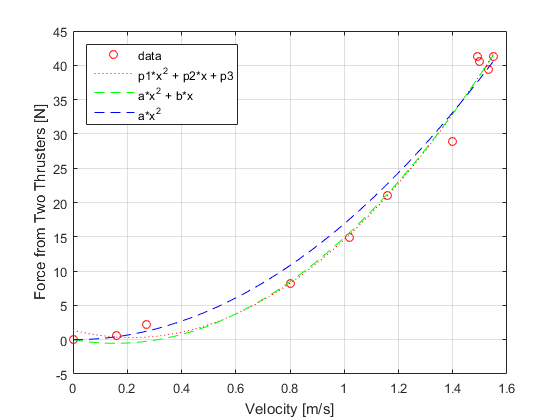
\includegraphics[width=0.75\linewidth]{quad_drag_surge.png}
\caption{Experimental identification of surge drag characteristics.}
\label{f:drag_surge}
\end{figure}

\begin{figure}[htbp]
\centering
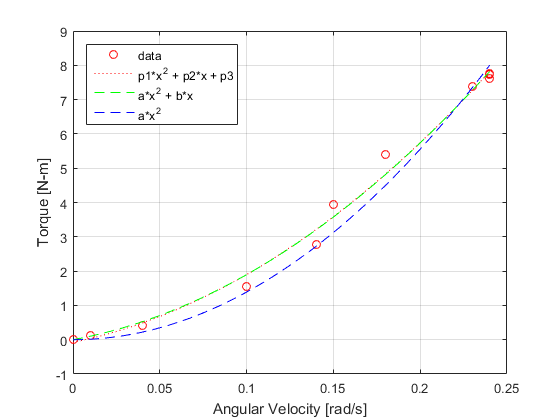
\includegraphics[width=0.75\linewidth]{quad_drag_yaw.png}
\caption{Experimental identification of yaw drag characteristics.}
\label{f:drag_yaw}
\end{figure}

\subsubsection{Linear Thrust Saturation}
Another important aspect of the system that can be represented is the limitation of the available control thrust. The bollard test data in Figure~\ref{f:tcurve} suggest the maximum forward thrust for each thruster is \unit[20]{N} and the maximum reverse thrust is \unit[-12]{N}.  

For surge force ($X_c$), this would result it maximum forward thrust of \unit[40]{N} and a minimum forward thrust of \unit[-12]{N}.

For yaw torque ($N_c$), this would result in a maximum of \unit[14]{Nm} - based on a distance between the two thrusters of \unit[0.88]{m}.

 
\subsubsection{Nonlinear Thrust Curve}
The input to the USV is a motor command.  This command is a normalized value ($\{-1.0,1.0\}$) sent to the speed controller for the electric motor.  This results in a thrust force for each thruster.  The experimental results in Figure~\ref{f:tcurve} and Table~\ref{t:tcurve} illstrate this nonlinear relationship.

\begin{figure}[htbp]
\centering
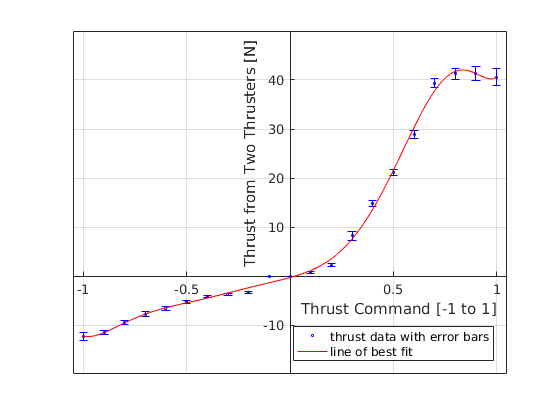
\includegraphics[width=0.9\linewidth]{thrust_cmd_relationship.png}
\caption{Relationship between thrust command a total measured thrust force (two thrusters). The ``line of best fit'' is a spline fit of the data.}
\label{f:tcurve}
\end{figure}

\begin{table}[hbt!] 
\renewcommand{\arraystretch}{1.2}
\caption{Relationship between measured thrust and thrust command for a single thruster.  }
\label{t:tcurve}
\centering
\csvautotabular{tcurve.csv}
\end{table}

We could implement this in at least two different ways.  We could use a table lookup method to interpolate between the discrete data points in Table~\ref{t:tcurve}.  For the purposes of the simulated USV model, this method would likely provide better agreement with the vehilce behavior.

Alternatively, we could fit the data with a function.  The generalized logitic function,
\begin{equation}
Y(x) = A + \frac{K-A}{ \left(C + \exp{(-B(x-M))} \right)^{1/\nu} },
\end{equation}
is a good candidate.  Because the thrust curve is not symmetric, we need to fit two curves---one for forward thrust and one for reverse thrust.  The resulting thruster curve model in Figure~\ref{f:tcurve_both} uses the parameters in Table~\ref{t:tcurvefit}.

\begin{figure}[htbp]
\centering
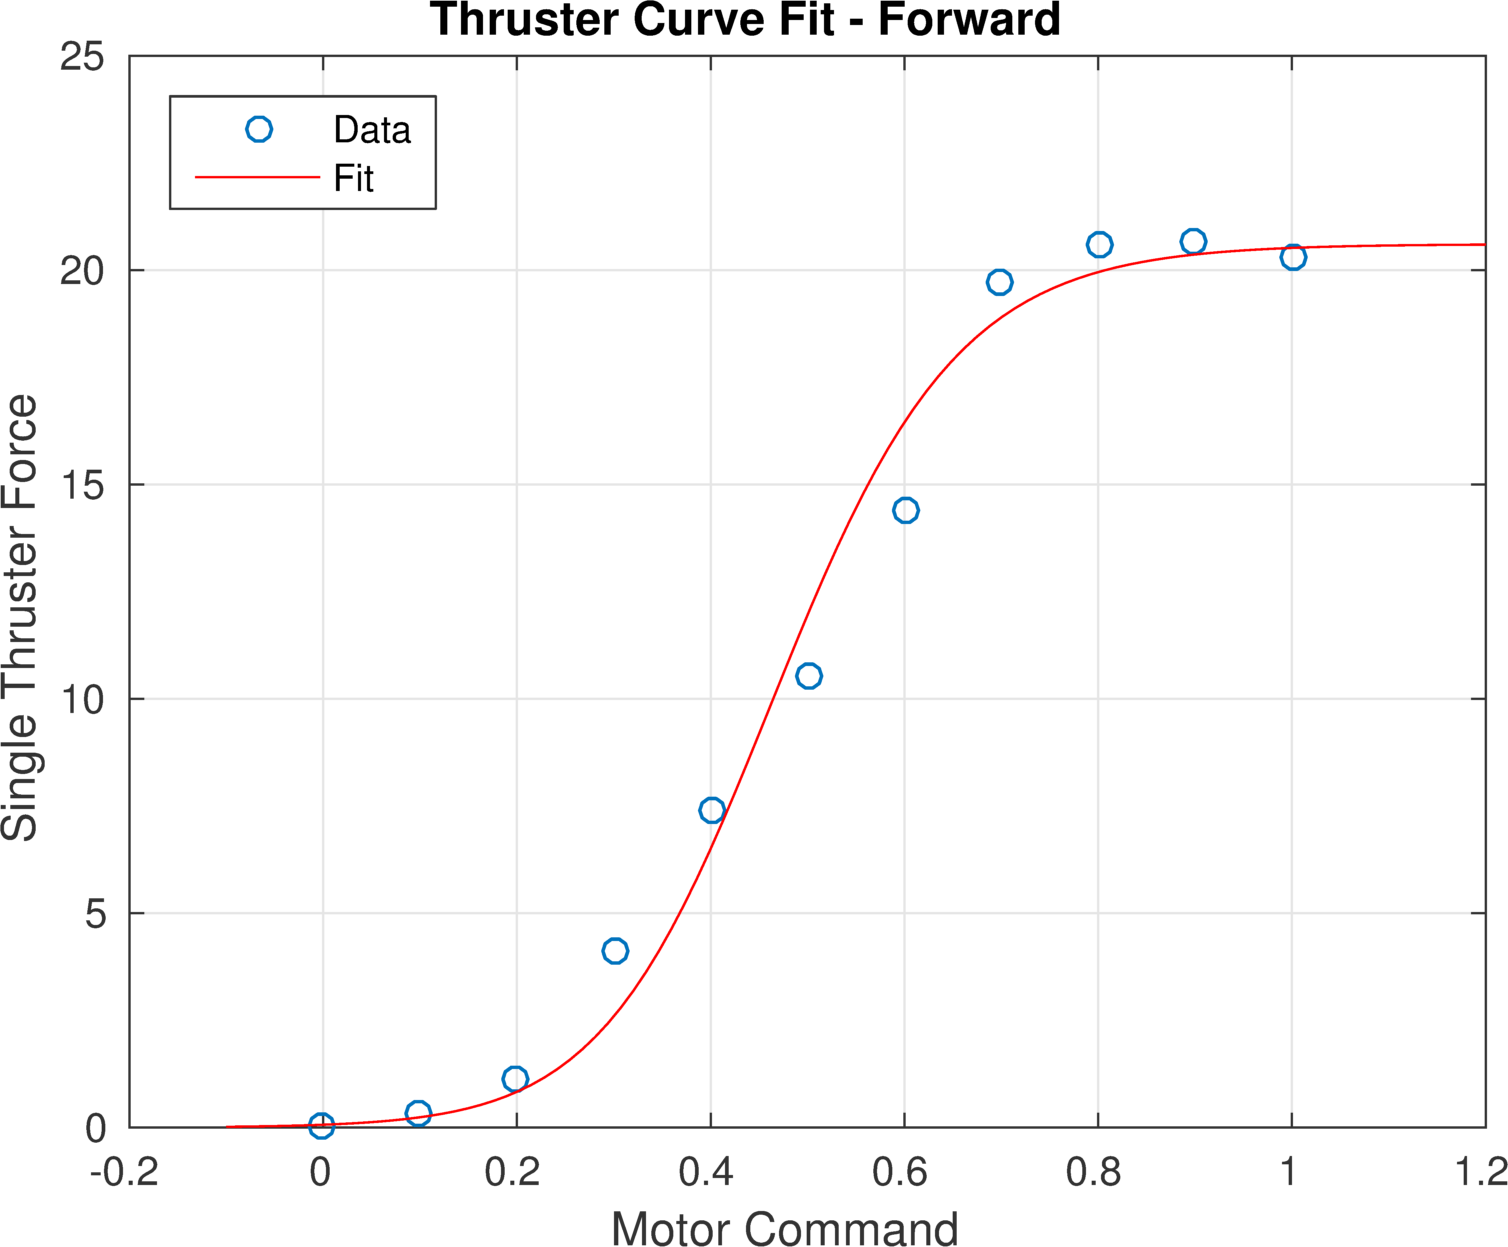
\includegraphics[width=0.7\linewidth]{tcurve_pos.png}
\caption{Thrust curve model for forward thrust - single thruster.}
\label{f:tcurve_pos}
\end{figure}

\begin{figure}[htbp]
\centering
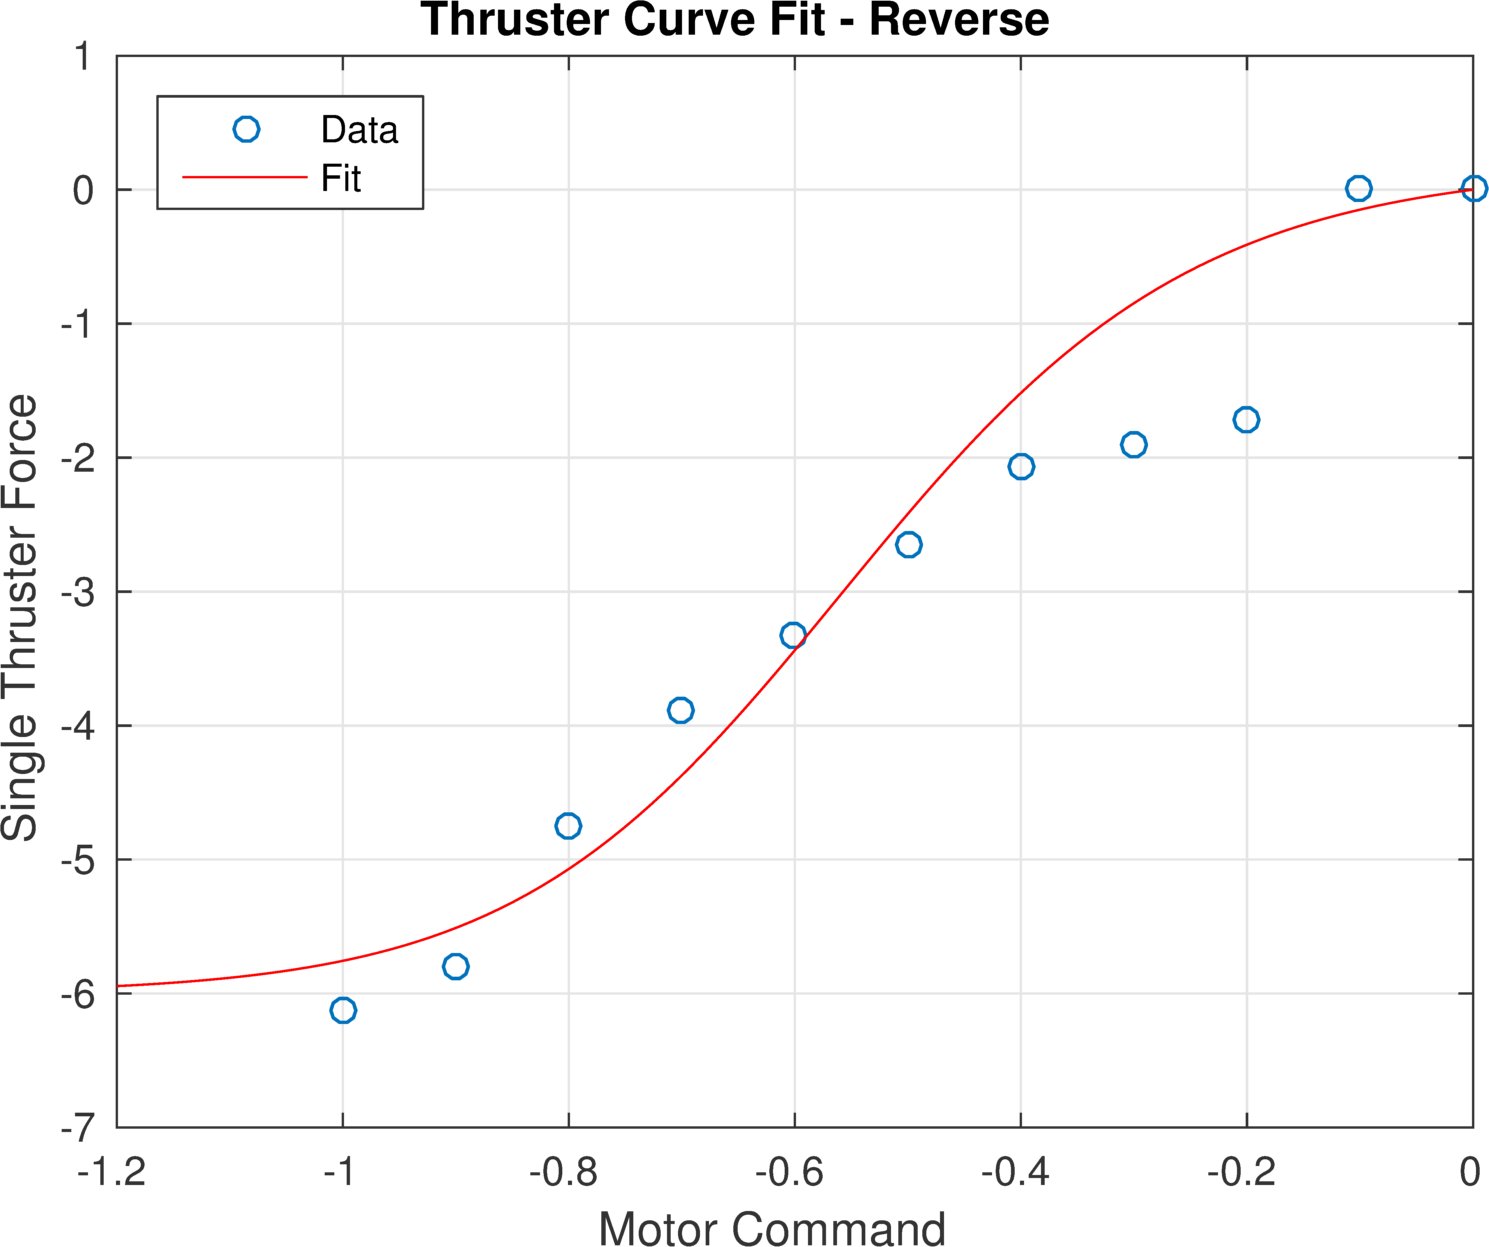
\includegraphics[width=0.7\linewidth]{tcurve_neg.png}
\caption{Thrust curve model for reverse thrust - single thruster.}
\label{f:tcurve_neg}
\end{figure}

\begin{figure}[htbp]
\centering
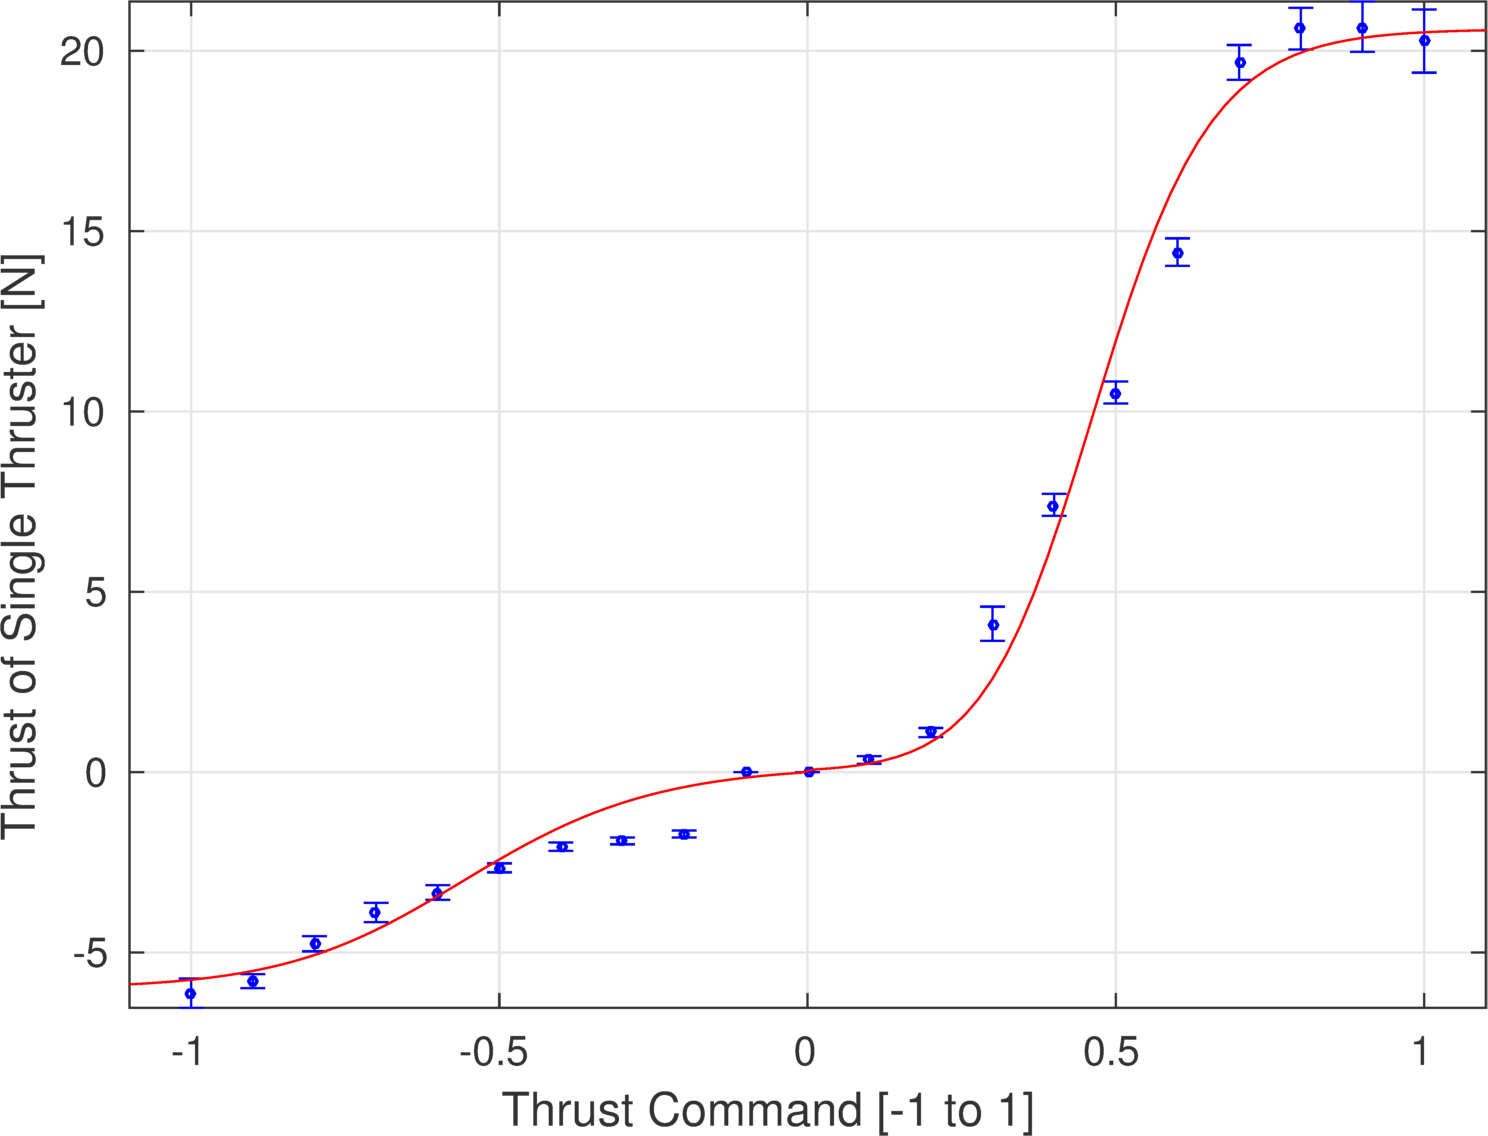
\includegraphics[width=0.7\linewidth]{tcurve_both.png}
\caption{Thrust curve model, generalized logistic functions, for forward and reverse thrust - single thruster.}
\label{f:tcurve_both}
\end{figure}


\begin{table}[hbt!] 
\renewcommand{\arraystretch}{1.2}
\caption{Generalized logistic function parameters for curve fit.}
\label{t:tcurvefit}
\centering
\csvautotabular{tcurvefit.csv}
\end{table}

\clearpage



\section{Maneuvering Models}
\subsection{Nonlinear Maneuvering Model based on Second-order Modulus Functions}\label{s:nonlinearmodel}
This model contains second-order (linear and quadratic) terms for the dissipative terms. In this section we follow the notation and process detailed in \cite{fossen11handbook}, Chapter 7. The horizontal-plane maneuvering model uses the state vector $\bm{\nu}=[u,v,r]^T$ where the velocities $u$, $v$ and $r$ are in the surge, sway and yaw directions respectively.  The velocities are considered to be relative to an irrotational constant ocean current.  The nonlinear maneuvering equations from \cite{fossen11handbook} are
\begin{equation}
\underbrace{\bm{M}_{RB}\dot{\bm{\nu}}+\bm{C}_{RB}(\bm{\nu})\bm{\nu}}_\text{rigid-body forces} +
\underbrace{\bm{M}_A\dot{\bm{\nu}}_r + \bm{C}_A(\bm{\nu}_r)\bm{\nu}_r + 
\bm{D}(\bm{\nu}_r)\bm{\nu}_r}_\text{hydrodynamic forces}
= \bm{\tau}+\bm{\tau}_{wind}+\bm{\tau}_{waves}
\label{e:fossenmodel}
\end{equation}
where $\bm{\nu}_r$ is the velocity vector relative to an irrotational water current $\bm{\nu}_c$, i.e., $\bm{\nu}=\bm{\nu}_r+\bm{\nu}_c$.  The rigid body kinetics are represented by the rigid body mass $\bm{M}_{RB}$ 
\begin{equation}
\bm{M}_{RB}= \left[ 
\begin{array}{ccc}
m & 0 & 0 \\
0 & m & m x_g \\
0 & m x_g & I_z 
\end{array} \right],
\end{equation}
where $m$ is the mass of the vehicle, $I_z$ is the moment of inertia about the body-centered z-axis and $x_g$ is distance along the x-axis from the origin of the body-centered frame to the center of gravity of the vessel.  The second rigid body term is the Coriolis-centripetal matrix,
\begin{equation}
\bm{C}_{RB}(\bm{\nu})= \left[ 
\begin{array}{ccc}
0 & 0 & -m(x_gr+v) \\
0 & 0 & mu \\
m(x_gr+v) & -mu  & 0 
\end{array} \right].
\end{equation}
Note that $\bm{C}_{RB}(\bm{\nu})$ is skew-symmetric, i.e., $\bm{C}_{RB}(\bm{\nu})=-\bm{C}_{RB}^T(\bm{\nu})$.  The hydrodynamic effects are represented by the added mass matrix
\begin{equation}
\bm{M}_{A}= \left[ 
\begin{array}{ccc}
-X_{\dot{u}} & 0 & 0 \\
0 & -Y_{\dot{v}} & -Y_{\dot{r}} \\
0 & -Y_{\dot{r}} & -N_{\dot{r}} 
\end{array} \right].
\end{equation}
and the Coriolis-centripetal matrix for the added mass
\begin{equation}
\bm{C}_{A}(\bm{\nu}_r)= \left[ 
\begin{array}{ccc}
0 & 0 & Y_{\dot{v}}v_r+Y_{\dot{r}}r \\
0 & 0 & -X_{\dot{u}}u_r\\
 -Y_{\dot{v}}v_r - Y_{\dot{r}}r& X_{\dot{u}}u_r & 0 
\end{array} \right].
\end{equation}
It is worth noting that $\bm{C}_A$ includes the nonlinear Munk moment (see \cite{fossen11handbook} p.121).  Following \cite{fossen11handbook} the SNAME notation for the hydrodynamic derivatives.

The linear and quadratic drag terms
\begin{equation}
\bm{D}(\bm{\nu}_r)= \left[ 
\begin{array}{ccc}
X_u + X_{u|u|}|u| & 0 & 0 \\
0 & Y_v + Y_{v|v|}|v| & Y_r+Y_{r|r|}|r|\\
0 & N_v + N_{v|v|}|v| & N_r+N_{r|r|}|r|
\end{array} \right].
\end{equation}

Equivalently we can express the same model in non-matrix form, where the speed equation in the surge direction is 
\begin{equation}
\underbrace{m \dot{u}}_\text{RB inertia}  
- \underbrace{m x_g r^2}_\text{RB centripetal}
- \underbrace{mvr}_\text{RB Coriolis}
=
\underbrace{X_{\dot{u}} \dot{u}_r}_\text{AM inertia}
+ \underbrace{Y_{\dot{v}}v_r r}_\text{AM Coriolis}
+ \underbrace{Y_{\dot{r}}r^2}_\text{AM centripetal}
+ \underbrace{X_u u + X_{u|u|}|u|u}_\text{Drag} 
+ \underbrace{\tau}_\text{Thrust}
\label{e:fullu}
\end{equation}
and the coupled steering questions in the sway direction 
\begin{equation}
\underbrace{m \dot{v} + m x_g \dot{r}}_\text{RB inertia}  
+ \underbrace{m ur}_\text{RB Coriolis}
- \underbrace{Y_{\dot{v}}\dot{v} - Y_{\dot{r}}\dot{r}}_\text{AM inertia}
=
+ \underbrace{Y_v v + Y_{v|v|}|v|v}_\text{Drag} 
+ \underbrace{Y_r r + Y_{r|r|}|r|r}_\text{Coupled Drag} 
\label{e:fullv}
\end{equation}
and yaw directions 

\begin{equation}
\underbrace{I_z \dot{r} + m x_g \dot{v}}_\text{RB inertia}  
+ \underbrace{m x_g ru}_\text{RB Coriolis}
- \underbrace{Y_{\dot{r}}\dot{v} - N_{\dot{r}}\dot{r}}_\text{AM inertia}
- \lefteqn{\overbrace{\phantom{Y_{\dot{v}}v_r u + X_{\dot{u}}u_r v}}^\text{Monk Moment}}
\underbrace{Y_{\dot{v}}v_r u + X_{\dot{u}}u_r v - Y_{\dot{r}}ru}_\text{AM Coriolis}
- \underbrace{N_v v + N_{v|v|}|v|v}_\text{Coupled Drag} 
+ \underbrace{N_r r + N_{r|r|}|r|r}_\text{Drag} 
= 
+ \underbrace{\tau}_\text{Torque}
\label{e:fullr}
\end{equation}

\pagebreak
\subsection{Sonnenburg Model}

The models described in \cite{sonnenburg10control} and \cite{sonnenburg13modeling} can be categorized as 
\begin{enumerate}
\item {\bf White Box} formulated with both the model structure and constituent parameters with physical meaning.  This model proposed with Fossen model presented in Section~\ref{s:nonlinearmodel}.  In theory, the parameter values for this model could be estimated from first principles, from analytic methods such as strip theory or numerical/CFD methods such as validated vaval architecture codes.  Although Sonnenburg presents the model structure and parameters, no estimate of the physical parameters is provided. 
\item {\bf Grey Box, Physical Model} where the model structure and model parameters are identical to the White Box model, but where system identification is used to estimate the physical parameters from experimental measurements.   No parameter estimates are provided.
\item {\bf Grey Box, Semi-Physical Model} formulated with a linear, state-space model structure where the model parameters cannot be mapped to physical parameters.  In this case Sonnenburg does provide empirical estimates of the non-physical model parameters.
\end{enumerate}
\cite{sjoberg95nonlinear,nugroho18comparison}


\subsubsection{Nonlinear Model}
The nonlinear model has the same terms maneuvering presented in Section~\ref{s:nonlinearmodel} with
\begin{enumerate}
\item the assumption that the water current velocity can be neglected so that the velocity relative to the water is equivalent to the velocity in the fixed frame, i.e., $\bm{\nu}=\bm{\nu}_r$.
\item the thrust ($\unit[\delta T]{\%}$) and steering angle ($\unit[\delta r]{degrees}$) are the only external forces and that they are coupled to all three degrees-of-freedom.
\end{enumerate}
We reproduce that physical, nonlinear model as
\begin{IEEEeqnarray}{C}
  \label{e:sonnenphysical}
  \IEEEyesnumber
  \IEEEyessubnumber*
\left[ 
\begin{array}{ccc}
m-X_{\dot{u}}& 0 & 0 \\
0 & m - Y_{\dot{v}} & (m x_g) -Y_{\dot{r}}  \\
0 &  (m x_g) -Y_{\dot{r}} & I_z -N_{\dot{r}} 
\end{array}
\right]
\left[
\begin{array}{c}
\dot{u}\\
\dot{v}\\
\dot{r}
\end{array}
\right]
+  \\
\left[ 
\begin{array}{ccc}
0 & 0 & -m(x_gr+v) + (Y_{\dot{v}}v+Y_{\dot{r}}r) \\
0 & 0 & mu -X_{\dot{u}}u \\
m(x_gr+v) -(Y_{\dot{v}}v + Y_{\dot{r}}r) & -mu +  X_{\dot{u}}u  & 0 
\end{array}
\right]
\left[
\begin{array}{c}
u\\
v\\
r
\end{array}
\right]
+ \\
\left[ 
\begin{array}{ccc}
X_u + X_{u|u|}|u| & 0 & 0 \\
0 & Y_v + Y_{v|v|}|v| & Y_r+Y_{r|r|}|r|\\
0 & N_v + N_{v|v|}|v| & N_r+N_{r|r|}|r|
\end{array} \right]
\left[
\begin{array}{c}
u\\
v\\
r
\end{array}
\right]
 \\
= \left[
  \begin{array}{c}
    X_{\mathrm{cntrl}}(\delta r, \delta T) \\
    Y_{\mathrm{cntrl}}(\delta r, \delta T) \\
    N_{\mathrm{cntrl}}(\delta r, \delta T)
  \end{array}
  \right].    
\end{IEEEeqnarray}


\noindent
Equivalently,
\begin{IEEEeqnarray*}{rCL}
    \IEEEyesnumber
  \underbrace{m \dot{u}}_\text{RB inertia}
- \underbrace{X_{\dot{u}} \dot{u}}_\text{AM inertia}
- \underbrace{m x_g r^2}_\text{RB centripetal}
- \underbrace{mvr}_\text{RB Coriolis}
+ \underbrace{Y_{\dot{v}}v r}_\text{AM Coriolis}
+ \underbrace{Y_{\dot{r}}r^2}_\text{AM centripetal}
- \underbrace{\left(X_u u + X_{u|u|}|u|u\right)}_\text{Nonlinear Drag} 
& = & \; \; \;
\\
\underbrace{X_{\text{cntrl}}(\delta r, \delta T)}_\text{Control}
 \; \; & &   \IEEEyessubnumber
\\
\underbrace{m \dot{v} + m x_g \dot{r}}_\text{RB inertia}  
- \underbrace{Y_{\dot{v}}\dot{v} - Y_{\dot{r}}\dot{r}}_\text{AM inertia}
+ \underbrace{m ur}_\text{RB Coriolis}
- \underbrace{X_{\dot{u}} u r}_\text{AM Coriolis}
+ \underbrace{Y_v v + Y_{v|v|}|v|v}_\text{Drag} 
+ \underbrace{Y_r r + Y_{r|r|}|r|r}_\text{Coupled Drag}
& = & \; \; \;
\\
\underbrace{Y_{\text{cntrl}}(\delta r, \delta T)}_\text{Control}
 \; \; & &   \IEEEyessubnumber
\\
\underbrace{I_z \dot{r} + m x_g \dot{v}}_\text{RB inertia}  
- \underbrace{\left(Y_{\dot{r}}\dot{v} + N_{\dot{r}}\dot{r}\right)}_\text{AM inertia}
+ \underbrace{m x_g ru  }_\text{RB Coriolis}
- \lefteqn{\overbrace{\phantom{Y_{\dot{v}}v u + X_{\dot{u}}u v}}^\text{Monk Moment}}
\underbrace{Y_{\dot{v}}v u + X_{\dot{u}}u v - Y_{\dot{r}}ru}_\text{AM Coriolis}
- \underbrace{N_v v + N_{v|v|}|v|v}_\text{Coupled Drag} 
+ \underbrace{N_r r + N_{r|r|}|r|r}_\text{Drag} 
& = & \; \; \;
\\
\underbrace{N_{\text{cntrl}}(\delta r, \delta T)}_\text{Control}
 \; \; & &   \IEEEyessubnumber
\end{IEEEeqnarray*}


\subsubsection{Linearized State-Space Model}

The physical model (\ref{e:sonnenphysical}) is a standard adaptation of Fossen and represents a common form of the maneuvering model based on physically meaningful model parameters.  However, the parameters of this model are neither calculated or estimated from data.  Instead the majority of the model complexity (coupling and off-diagonal terms, etc.) are neglected in the formulation of a semi-physical model for which the parameters of the model are observable from on-water experiments.  The resulting linearized state-space model can be expressed as
\begin{IEEEeqnarray}{C}
\label{e:statespace}
\left[
\begin{array}{c}
\dot{u}\\
\dot{v}\\
\dot{r}
\end{array}
\right]
=
\left[ 
\begin{array}{ccc}
  a & 0 & 0 \\
  0 & a_{11} & a_{12} \\
  0 & a_{21} & a_{22} 
\end{array}
\right]
\left[
\begin{array}{c}
u\\
v\\
r
\end{array}
\right]
+
\left[ 
\begin{array}{cc}
b & 0 \\
0 &  b_1 \\
0 &  b_2
\end{array} \right]
\left[ 
\begin{array}{cc}
  \delta T \\
  \delta r
  \end{array}
  \right].    
\end{IEEEeqnarray}
This model form is then used as the basis for system identification leading to the parameter estimates reproduced in Figure~\ref{f:table16}.

\begin{figure}[htbp]
\centering
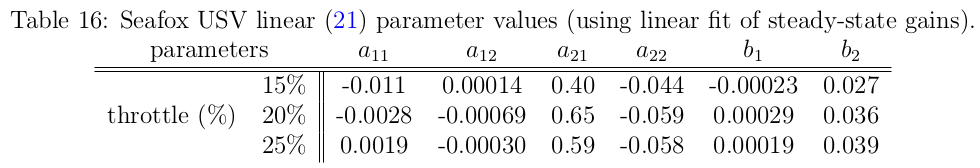
\includegraphics[width=0.90\linewidth]{sonnenburg_table16.png}
\caption{Source \cite{sonnenburg10control}.}
\label{f:table16}
\end{figure}

Conceptually, the simplification from the physical model (\ref{e:sonnenphysical}) to the semi-physical state-space model (\ref{e:statespace}) could be possible with the following assumptions: 
\begin{itemize}
\item Surge centripetal and Coriolis terms are neglected.
\item Yaw Coriolis terms are neglected, with the exception of the $X_{\dot{u}}uv$ term which may contribute to $a_{21}$. (There are no yaw centripetal terms.)
\item Rigid-body and added mass inertial parameters are lumped together and can not be independently specified or estimated.
\item The origin of the body-centered reference frame is collocated with the center of mass so that $x_g = 0$ and off diagonal terms of the inertial matrix are negligible.
\item Drag forces are linear - quadratic terms are negligible for small changes from the setpoint.
\item The parameters of the model in (\ref{e:statespace}) are estimated for different throttle setting as shown in Figure~\ref{f:table16}.  The functional relationship between the parameters and $u$ is not estimated.
\end{itemize}

For the purposes of comparison we re-write (\ref{e:statespace}) with the state transition matrix on the left side and the input matrix on the right, 
\begin{IEEEeqnarray}{C}
\label{e:statespace2}
\left[
\begin{array}{c}
\dot{u}\\
\dot{v}\\
\dot{r}
\end{array}
\right]
-
\left[ 
\begin{array}{ccc}
  a & 0 & 0 \\
  0 & a_{11} & a_{12} \\
  0 & a_{21} & a_{22} 
\end{array}
\right]
\left[
\begin{array}{c}
u\\
v\\
r
\end{array}
\right]
=
\left[ 
\begin{array}{cc}
b & 0 \\
0 &  b_1 \\
0 &  b_2
\end{array} \right]
\left[ 
\begin{array}{cc}
  \delta T \\
  \delta r
  \end{array}
  \right]    
\end{IEEEeqnarray}


And we re-write the physical model  (\ref{e:sonnenphysical}), applying the the implicit assumption necessary to adopt the state-space form, we express this as
\begin{IEEEeqnarray}{C}
  \label{e:physicalcompare}
  \IEEEyesnumber
  \IEEEyessubnumber*
\left[ 
\begin{array}{ccc}
m-X_{\dot{u}}& 0 & 0 \\
0 & m - Y_{\dot{v}} &  -Y_{\dot{r}}  \\
0 &  -Y_{\dot{r}} & I_z -N_{\dot{r}} 
\end{array}
\right]
\left[
\begin{array}{c}
\dot{u}\\
\dot{v}\\
\dot{r}
\end{array}
\right]
+  \\
\left[ 
\begin{array}{ccc}
0 & 0 & 0 \\
0 & 0 & (m -X_{\dot{u}})u \\
0 & -(m- X_{\dot{u}})u  & 0 
\end{array}
\right]
\left[
\begin{array}{c}
u\\
v\\
r
\end{array}
\right]
+ \\
\left[ 
\begin{array}{ccc}
X_u & 0 & 0 \\
0 & Y_v  & Y_r\\
0 & N_v  & N_r
\end{array} \right]
\left[
\begin{array}{c}
u\\
v\\
r
\end{array}
\right]
 \\
= \left[
  \begin{array}{c}
    X_{\mathrm{cntrl}}(\delta r, \delta T) \\
    Y_{\mathrm{cntrl}}(\delta r, \delta T) \\
    N_{\mathrm{cntrl}}(\delta r, \delta T)
  \end{array}
  \right]    
\end{IEEEeqnarray}

We observe that the state-space model (\ref{e:statespace2}) used as the model form for system identification has only 5 parameters on the left hand side, while the physical model (\ref{e:physicalcompare}) has 11 parameters on the left hand side.  This suggests that the semi-physical model determined by the empirical identification cannot be meaningfully related to the physical model---that the model identification does not provide physically meaningful parameter estimates.  This greatly reduces the utility of the model by implying that it is only applicable to this one system under the specific operating conditions.  The lack of physical semantics in the model make it challenging (impossible?) to use the model for to approximate the dynamics of similar craft since there is no clear way to adjust the parameters based on first principles or comparisons between systems.

\subsection{Nonlinear Model of Blanke}
As reported by \cite{fossen94guidance}, this model ``retains the most important terms for steering and propulsion''.  Formulating these equations for a rudder-less vessel, the speed equation becomes
\begin{equation}
(m-X_{\dot{u}}) \dot{u} = X_{u|u|}|u|u + (m+X_{vr})vr + (mx_g+X_{rr})r^2 + \tau
\label{e:blankeu}
\end{equation}
Comparing (\ref{e:fullu}) and (\ref{e:blankeu}), noting that $Y_{\dot{v}}$ from  (\ref{e:fullu}) is equivalent to $X_{vr}$ in (\ref{e:blankeu}),  we can see that the only difference between these models is that the full model in (\ref{e:fullu}) includes both linear and quadratic drag terms, while Blanke's model includes only a quadratic term.  The linear term is important because it forces the system to converge to zero surge.  Furthermore, results of other experiments suggest that the drag is not purely quadratic.  

Blanke's steering model in sway, without rudder terms, is
\begin{equation}
(m-Y_{\dot{v}}) \dot{v} + (m x_g - Y_{\dot{r}}) \dot{r}
=
-(m -Y_{ur})ur + Y_{uv}uv + Y_{v|v|}|v|v + Y_{|v|r}|v|r.
\label{e:blankev}
\end{equation}
Comparing (\ref{e:fullv}) and (\ref{e:blankev}) we note the following differences
\begin{itemize}
\item The ``Coupled Drag'' term in (\ref{e:fullv}) is neglected in the Blanke model. \hl{What is the affect of neglecting these coupled drag terms? Appears fairly commonly in simplified models.}
\item The linear component of cross-flow drag (\ref{e:fullv}) is neglected in the Blanke model
\item The following second-order cross-coupling terms are present in Blanke that are not represented in  (\ref{e:fullv})
  \begin{itemize}
    \item $Y_{ur}ur$ - which appears as an added mass Coriolis term
    \item $Y_{uv}uv$
    \item $Y_{|v|r}|v|r$
    \item \hl{What is the consequence of neglecting these? 
Ditto for the yaw eqn.}
  \end{itemize}
\end{itemize}
The steering equation for yaw is
\begin{equation}
(m x_g - N_{\dot{v}})\dot{v} + (I_z - N_{\dot{r}})\dot{r}
=
-(m x_g - N_{ur})ur + N_{uv}uv + N_{v|v|}|v|v + N_{|v|r}|v|r
\label{e:blanker}
\end{equation}
\hl{What/Why is the quadratic yaw drag expressed as $N_{v|v|}|v|v$?  Seems like it would be $N_{r|r|}|r|r$.}

\noindent
Comparing (\ref{e:fullr}) and (\ref{e:blanker}), we note that the Monk moment has been collapsed into a single term $N_{uv}uv$ in (\ref{e:blanker}).  We note the following differences
\begin{itemize}
\item The ``Coupled Drag'' term in (\ref{e:fullr}) is neglected in the Blanke model
\item The linear component of yaw drag (\ref{e:fullv}) is neglected in the Blanke model
\item The second-order cross-coupling term $N_{|v|r}|v|r$ is present in Blanke model and not represented in\eref{e:fullr}.
\end{itemize}

\subsection{Simplified Model of Blanke from \cite{caccia08practical}}
In \cite{caccia08practical} the Blanke model is used, with the addition of linear drag terms, and the following assumptions are made:
\begin{itemize}
\item Speed: Surge
  \begin{itemize}
  \item Added mass in surge ($X_{\dot{u}}$) is negligible - less than 5\% of vessel mass.  This seem reasonable, but is not really necessary since the mass and added mass are lumped together in the identification.
  \item The Coriolis terms $(m+X_{vr})vr$, both rigid body and added mass contributions, are negligible because the sway speed is negligible.  \hl{This would seem to limit the sideslip.}  The experiments in \cite{sonnenburg10control}suggest the sideslip would be an important component for this type of vehicle.
  \item The centripetal terms $(mx_g+X_{rr})r^2$ are neglected on the assumption of a low turn rate.  This is probably reasonable?
  \end{itemize}
\item Steering: Sway and Yaw
  \begin{itemize}
  \item Added mass in both directions is neglected.  Again, probably not necessary since the identification estimates the combination of rigid body and added mass.
  \item Although the author's don't make it explicit(!), they neglect the rigid body and added mass coupling terms  \hl{I believe this is equivalent to assuming that the principle axes of inertia for the vessel (the body-centered coordinate frame) are co-located with the center of mass of the vessel.}
    \begin{itemize}
    \item $(m x_g - Y_{\dot{r}})\dot{r}$ in the sway equation
    \item $(m x_g - N_{\dot{v}})\dot{v}$ in the yaw equation
    \end{itemize}
  \item Again, this is not explicit, but the authors omit the Coriolis terms, both rigid body and added mass, $-(mx_g-N_{ur})ur$. The reason for omission is not provided in the text.
  \item The ``coupled drag terms are neglected because $v$ and $r$ are typically small''.  We can only assume they are referring to the following terms - \hl{Are these correctly identified as ``coupling drag terms''?  Are they negligible?}
    \begin{itemize}
    \item $Y_{uv}uv$ and $Y_{|v|r}|v|r$ are negligible in sway
    \item $N_{uv}uv$ and $N_{|v|r}|v|r$ are negligible in yaw
    \end{itemize}
   \item The quadratic term $N_{|v|v}|v|v$ in the Blanke model is substituted with a linear and quadratic term as a function of yaw, $N_r r+N_{|r|r}|r|r$. \hl{As indicated previously, I'm not clear whey this term is related to the sway velocity in the first place.}
  \end{itemize}
\end{itemize}
For our vessel this would be equivalent to the following speed and steering equations
\begin{equation}
m\dot{u} = X_u u X_{|u|u}|u|u + \tau
\end{equation}
\begin{equation}
(m) \dot{v}
=
-(m -Y_{ur})ur + Y_v v + Y_{v|v|}|v|v .
\label{e:blanke2v}
\end{equation}
\begin{equation}
I_z\dot{r}
=
 N_r r + N_{r|r|}|r|r + \tau
\label{e:blanke2r}
\end{equation}
This model is greatly simplified. \hl{Us such a high degree of simplification justified?}

\subsection{\cite{muske08identification}}
The model in \cite{muske08identification} supposedly comes from  \cite{fossen94guidance} (although I haven't found it yet).  This model includes a power-law drag model in each direction, combined rigid body and added mass terms and (unlike the simplified Blanke model from \cite{caccia08practical}) includes the Coriolis terms.  The equations of motion are
\begin{eqnarray}
m_{11}\dot{u} - m_{22}vr + d_1 u^{\alpha_1} = \tau_{Thrust} \\
m_{22}\dot{v} +  m_{11}ur + d_2 u^{\alpha_2} = 0\\
m_{33}\dot{r} + (m_{22}-m_{11})uv + d_3 u^{\alpha_3} = \tau_{Torque} \\
\end{eqnarray}
Comparing this model to the nonlinear maneuvering model in \eref{e:fullu} \eref{e:fullv} \eref{e:fullr} we see that
\begin{itemize}
\item Rigid body mass and added mass are combined in all terms
\item They assume the body-axis and center of mass are collocated
\item All centripetal terms are neglected
\item Drag modeled as a power law, which may be more general (with the same number of parameters) as the linear+quadratic model.
\item There are some additional assumptions here to make this work out - i.e., deriving this from the original nonlinear model.
\end{itemize}

\subsection{Thrust Model}
Two options:

Assume thrust is independent of speed (as done in the Caccia papers).

Or assume and unknown, linear decrease in thrust with speed.
\[
T = T_o (1-au)
\]
where $a$ is the linear speed reduction
\subsection{Speed model}
Consider the surge state of the model above where
\begin{equation}
\underbrace{m \dot{u}}_\text{RB inertia}  
- \underbrace{m x_g r^2}_\text{RB centripetal}
- \underbrace{mvu}_\text{RB Coriolis}
=
\underbrace{X_{\dot{u}} \dot{u}}_\text{AM inertia}
+ \underbrace{Y_{\dot{v}}v_r r}_\text{AM Coriolis}
+ \underbrace{Y_{\dot{r}}r^2}_\text{AM centripetal}
+ \underbrace{X_u u + X_{u|u|}|u|u}_\text{Drag} 
+ \underbrace{T}_\text{Thrust}
\end{equation}
Following \cite{caccia08practical}, based on \cite{fossen94guidance}, we neglect the second-order centripetal terms
\begin{equation}
m \dot{u}
- mvu
=
X_{\dot{u}} \dot{u}
+ Y_{\dot{v}}v_r r
+ X_u u + X_{u|u|}|u|u
+ T
\end{equation}

For steady state forward motion ($\dot{u}=v=r=0$) in stationary water ($v_r=0$)
\begin{equation}
0 =
+ X_u u + X_{u|u|}|u|u
+ T
\end{equation}
We can estimate $X_u$ and $X_{u|u}$ from steady state forward motion trials with known thrust input by testing at a series of known forward speeds and measuring $u$.

Considering forward-only acceleration
\begin{equation}
m \dot{u}
=
X_{\dot{u}} \dot{u}
+ X_u u + X_{u|u|}|u|u
+ T
\end{equation}
we can identify the added mass ($X_{\dot{u}}$) by either estimating the initial acceleration (see \cite{sonnenburg10control}) or by examining the 'time constant' for such tests.

This leaves the coefficient $Y_{\dot{v}}$, related to the added-mass Coriolis force, as the single unknown.


\section{Proposed Model}

\subsection{Actuation Model}
The thrust provided by each motor is a function of the command input ($\alpha$) provided to the motor controller.  The total thrust applied to the vessel is twice the motor thrust, so
\begin{equation}
\tau_{thrust}= 2 (f(\alpha)).
\label{e:thrust}
\end{equation}

Torque is applied to the vessel by a torque command ($\beta$) applied equal and opposite to the two thrusters separated by a distance of $d$, so
\begin{equation}
\tau_{torque}= d (f(\beta)).
\label{e:torque}
\end{equation}

We assume that any lag between the command inputs and the resutling thurst and torque is small compared to the dynamics of the vessel.

\subsection{Maneuvering Model}
We start with the maneuvering model from \cite{fossen11handbook} Chapter 7, in (\ref{e:fossenmodel}---\ref{e:fullr}).  We make the following assumptions
\begin{itemize}
\item The center of mass of the vehicle and the origin of the principle axes are co-located.  Therefore $x_g$ can be neglected.
\item Centripetal terms can be neglected because of typically small yaw rates.
\item The coupled terms in the added mass matrix ($Y_{\dot{r}}$) are sufficiently small to be neglected.
\item The coupling in the drag matrix can be neglected.
\item The values for the mass ($m$) and inertia ($I_z$) of the vessel can be measured directly
\item For the purposes of model identification, the water current velocity is zero so that $\bm{nu}=\bm{nu}_r$.
\end{itemize}
Applying these assumptions, we can formulate the maneuvering model as follows.  The mass matrix becomes the diagonal matrix
\begin{equation}
\bm{M}= \left[ 
\begin{array}{ccc}
m-X_{\dot{u}} & 0 & 0 \\
0 & m-Y_{\dot{v}} & 0 \\
0 & 0 & I_z-N_{\dot{r}} 
\end{array} \right].
\end{equation}
The Coriolis matrix reduces to 
\begin{equation}
\bm{C}(\bm{\nu})= \left[ 
\begin{array}{ccc}
0 & 0 & -(m-Y_{\dot{v}})v \\
0 & 0 & (m-X_{\dot{u}})u \\
(m-Y_{\dot{v}})v & -(m-X_{\dot{u}})u  & 0 
\end{array} \right].
\end{equation}
The linear and quadratic drag matrix becomes
\begin{equation}
\bm{D}(\bm{\nu}_r)= \left[ 
\begin{array}{ccc}
X_u + X_{u|u|}|u| & 0 & 0 \\
0 & Y_v + Y_{v|v|}|v| & 0 \\
0 & 0  & N_r+N_{r|r|}|r|
\end{array} \right].
\end{equation}


\section{Model Identification Tests}
\subsection{Physical Measurements}
\begin{itemize}
\item Measure the mass ($m$) directly.  
\item Measure the moment of inertia ($I_z$) using a bifilar pendulum.
\end{itemize}

\subsection{Thrust Characterization}
Bollard tests in the tank to measure thrust force (at zero velocity) as a function of motor command.  Use a load cell to measure the steady state force generated by the thrusters when attached to the tank.  Measure the force at a number of thrust commands (e.g., 10 steps between 0-1.0 and -1.0-0).  Fit a curve to the resulting command vs. thrust relationship to identify the function in (\ref{e:thrust}).

\subsection{Steady-State Tests}
\begin{itemize}
\item Yaw: Measure the steady-state yaw rate at variety of torque inputs to identify the yaw drag terms. Direct estimate of $N_r$ and $N_{r|r|}$.
\item Surge: Measure the steady-state speed at a variety of thrust inputs to identify the drag terms. Direct estimate of $X_u$ and $X_{u|u|}$.
\end{itemize}


\subsection{Open-Loop Dynamic Tests}
\begin{itemize}
\item Yaw: Measure step response to torque to estimate added mass/inertia in yaw.  Direct estimate of $N_{\dot{r}}$.
\item Surge: Measure step response to forward thrust (with heading control?) to estimate added surge mass. Direct estimate of $X_{\dot{u}}$.
\end{itemize}

\subsection{Maneuvering Tests}
We are left with the following parameters to identify
\begin{itemize}
\item $Y_{\dot{v}}$: Added-mass in sway
\item $Y_v$ and $Y_{v|v|}$: Linear and quadratic drag in sway
\end{itemize}

We can isolate the drag parameters by performing ``turning circle'' tests there the vehicle is moved in a circle with constant speed and yaw rate.  Performing this test at different levels of thrust and torque should all for direct estimation of the linear and quadratic drag terms.

The last test is a set of step changes in speed and/or heading while executing the steady-state turning circle.  This should allow an estimate of $Y_{\dot{v}}$.

%\subsection{Verification}
%\subsection{Closed-Loop Dynamic Tests}

%\section{Ship Dynamics}
%Following \cite{fossen94guidance}, Ch 5.


%\section{Acknowledgments}

% standard IEEE bibliography style from:
% http://www.ctan.org/tex-archive/macros/latex/contrib/supported/IEEEtran/bibtex
%\bibliographystyle{../latex_ieee/IEEEtran}
\bibliographystyle{apalike}
% argument is your BibTeX string definitions and bibliography database(s)

\ifoverleaf
\bibliography{bbing_master}
\else
\bibliography{../latexlib/bib/bbing_master}
\fi

%\bibliography{./latex_ieee/IEEEabrv}

% if you will not have a photo at all:

% that's all folks

\end{document}


